\documentclass[a4paper,12pt]{report} %%%{article}

\usepackage{cmap} % searchable PDFs
\usepackage[T2A]{fontenc} % scalable fonts
\usepackage[utf8]{inputenc} % input in UTF8
\usepackage[english,russian]{babel} % dashes on linebreaks
\usepackage{indentfirst} % indents in paragraphs
\usepackage{amstext,amssymb,amsfonts,amsmath,mathtext,enumerate,float}
\usepackage[left=25mm,right=2cm,top=2cm,bottom=2cm,bindingoffset=0cm]{geometry}
\usepackage[unicode]{hyperref}
\usepackage{graphicx}
\usepackage{ulem} % strikethrough
\usepackage{verbatim} % multiline comments
\usepackage{hhline}

\usepackage{listings}
\usepackage{color}
 
\lstset{extendedchars=\true}
  
\definecolor{dkgreen}{rgb}{0,0.6,0}
\definecolor{gray}{rgb}{0.5,0.5,0.5}
\definecolor{mauve}{rgb}{0.58,0,0.82}
 
\lstset{ %
  columns=flexible,
%  language=C,                     % the language of the code
  basicstyle=\footnotesize\ttfamily,       % the size of the fonts that are used for the code
  numbers=left,                   % where to put the line-numbers
  numberstyle=\tiny\color{gray},  % the style that is used for the line-numbers
  stepnumber=1,                   % the step between two line-numbers. If it's 1, each line will be numbered
  numbersep=5pt,                  % how far the line-numbers are from the code
  backgroundcolor=\color{white},  % choose the background color. You must add \usepackage{color}
  showspaces=false,               % show spaces adding particular underscores
  showstringspaces=false,         % underline spaces within strings
  showtabs=false,                 % show tabs within strings adding particular underscores
%  frame=single,                   % adds a frame around the code
  rulecolor=\color{black},        % if not set, the frame-color may be changed on line-breaks within not-black text (e.g. comments (green here))
  tabsize=4,                      % sets default tabsize
  captionpos=b,                   % sets the caption-position to bottom
  breaklines=true,                % sets automatic line breaking
  breakatwhitespace=false,        % sets if automatic breaks should only happen at whitespace
  title=\lstname,                 % show the filename of files included with \lstinputlisting; also try caption instead of title
  keywordstyle=\color{blue},      % keyword style
  commentstyle=\color{dkgreen},   % comment style
  stringstyle=\color{mauve},      % string literal style
%  escapeinside={\%*}{*)},         % if you want to add LaTeX within your code
  mathescape=true,
  morekeywords={*,...},           % if you want to add more keywords to the set
  deletekeywords={...},           % if you want to delete keywords from the given language
  aboveskip=1em,
  belowskip=-1em
}


\usepackage{mathtools}
\newcommand{\defeq}{\vcentcolon=}
\newcommand{\eqdef}{=\vcentcolon}

\renewcommand{\contentsname}{Содержание} 
\setcounter{secnumdepth}{0}
\setcounter{tocdepth}{3}

% \linespread{1.3}
\sloppy % align=justify


\begin{document}

\newcommand{\Deltasigma}{\Delta_\alpha^\rho\sigma}

Рассмотрим $\sigma$ и $\Deltasigma$ и некоторое $s \in \sigma$. Хочется, зная $d(\sigma, s)$, сделать какие-то выводы о $d(\Deltasigma, s)$. Посмотрим, как может изменяться $d(\cdot, s)$ при изменениях первого аргумента.

Определим функцию $b(\sigma, s) = \{t \in \sigma \mid \exists \sigma' \subseteq \sigma : d(\sigma', s) \text{ определено, } t \in d(\sigma', s) \}$~--- те элементы $\sigma$, от которых ``может зависеть'' $s$. Если $d(\sigma, s)$ определено, то $b(\sigma, s) = d(\sigma, s)$; если $d(\sigma, s)$ не определено из-за недостающих зависимостей (назовём такую ситуацию ``недоопределённостью''), то $b(\sigma, s) = \varnothing$; если $d(\sigma, s)$ не определено из-за дублирующих зависимостей (назовём такую ситуацию ``переопределённостью''), то $b(\sigma, s)$ определено (и равно объединению всех подмножеств $\sigma$, являющихся ``хорошими'' контекстами).

Тогда при переходе от одного $\sigma$ к другому ситуация с определённостью $d(\cdot, s)$ может меняться следующим образом:

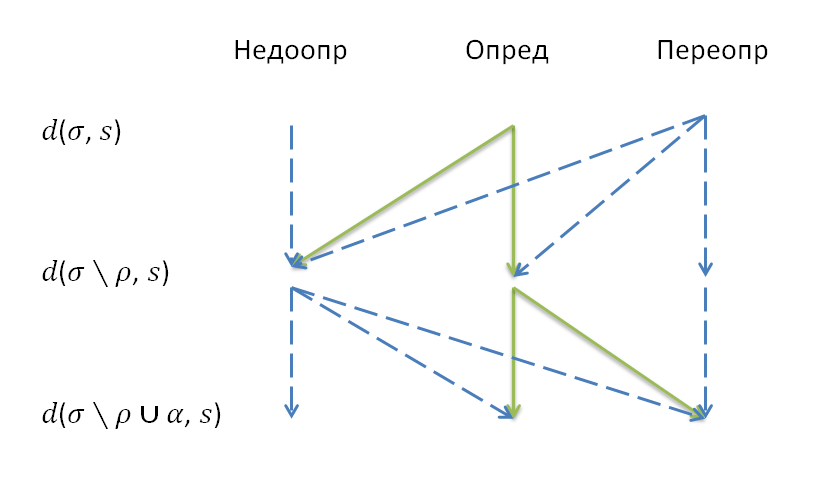
\includegraphics[scale=0.7]{compute_def_scheme}

Заметим, что для сплошных линий понятен критерий, в зависимости от которого изменится ситуация. В случае с вычитанием $\rho$ ситуация недоопределённости возникнет тогда и только тогда, когда $d(\sigma, s) \cap \rho \neq \varnothing$, в противном случае функция не только останется определённой, но и не изменит своего значения (по соответствующим аксиомам). Аналогично, в случае с добавлением $\alpha$ ситуация переопределённости возникнет тогда и только тогда, когда $b(\sigma, s) \cap \alpha \neq \varnothing$, в противном случае значение не изменится. Но если в первом случае $d(\sigma, s)$ известно и критерий можно проверить, то во втором применение критерия требует вычисления $d$ на каком-то новом множестве. Необходимо как-то понимать, может ли добавленное $\alpha$ внести неоднозначность в определение контекста. Как это проверить без вычисления, например, $d(\Deltasigma, s)$, пока непонятно.

\end{document}